%!TEX program = xelatex


\documentclass[xetex]{beamer}

\usepackage{amsmath,amsfonts,amsthm,amssymb}
\usepackage{graphicx,float,wrapfig}
\usepackage{subcaption}

\usepackage{natbib}
\usepackage[noend]{algpseudocode}
\usepackage{algorithm}
\usepackage{xspace}
\usepackage{subcaption}
\usepackage{theoremref}
\usepackage{thmtools}
\usepackage{thm-restate}
\usepackage{cleveref}


\usepackage[quiet]{fontspec}
\usepackage{xunicode}
\usepackage{xltxtra}
%\usepackage{graphicx}
\usepackage{stmaryrd}
\usepackage{xcolor}
%\usepackage{tikz}
%\usepackage{almslides}


\frenchspacing
\unitlength=0.01\textwidth
\thicklines
\urlstyle{sf}


\def\fern{407428}
\def\charcoal{4D4944}
\definecolor{DarkFern}{HTML}{\fern}
\definecolor{DarkCharcoal}{HTML}{\charcoal}
\colorlet{Fern}{DarkFern!85!white}
\colorlet{Charcoal}{DarkCharcoal!85!white}
\colorlet{LightCharcoal}{Charcoal!50!white}
\colorlet{AlertColor}{orange!80!black}
\colorlet{DarkRed}{red!70!black}
\colorlet{DarkBlue}{blue!70!black}
\colorlet{DarkGreen}{green!70!black}

\setbeamercolor{title}{fg=Fern}
\setbeamercolor{frametitle}{fg=Fern}
\setbeamercolor{normal text}{fg=black}

\defaultfontfeatures{
    Mapping=tex-text,
    Scale=MatchLowercase,
}
%\setsansfont{Optima}
%\setmonofont{Monaco}

%\def\heading{%
%  \large%
%  \fontspec[
%    Color=\fern,
%    Contextuals={WordInitial,WordFinal},
%    Alternate=1
%  ]{Hoefler Text Italic}%
%}

\newcommand{\junk}[1]{}

\setbeamertemplate{frametitle}
  {\begin{centering}\smallskip
   \insertframetitle\par
   \smallskip\end{centering}}

\setbeamercolor{block title}{fg=black,bg=Fern!25!white}
\setbeamercolor{block body}{fg=black,bg=Fern!25!white}

\setbeamercolor{notitle}{fg=black,bg=Fern!25!white}
\setbeamercolor{alerted text}{fg=AlertColor}
%% \setbeamercolor{palette primary}{fg=white,bg=black}
%% \setbeamercolor{palette secondary}{fg=white,bg=black}
%% \setbeamercolor{palette tertiary}{fg=white,bg=black}
\setbeamertemplate{itemize item}{$\bullet$}
\setbeamercolor{itemize item}{fg=Charcoal}

\setbeamertemplate{navigation symbols}{}
\setbeamertemplate{footline}[text line]{%
    \hfill\strut{%
        \scriptsize\sf\color{black!60}%
        \quad\insertframenumber%
    }%
    \hfill%
}


\captionsetup[subfigure]{labelformat=empty, labelsep=none}


\newcommand{\Algorithm}{{\small \textsf{CLUCB}}\xspace}
\newcommand{\AlgorithmPAC}{{\small \textsf{CLUCB-PAC}}\xspace}
\newcommand{\AlgorithmBud}{{\small \textsf{CSAR}}\xspace}
\newcommand{\Uniform}{{\small \textsf{UNI}}\xspace}
%\newcommand{\Problem}{{\small \textsf{ExpCMAB}}\xspace}
%\newcommand{\Problem}{{CPE}\xspace}
\newcommand{\Rew}{\varphi}
\newcommand{\E}{\mathbb E}

\renewcommand{\M}{\mathcal M}
\newcommand{\mmatch}{\mathcal M_{\mathsf{MATCH}}}
\newcommand{\mtop}{\mathcal M_{\mathsf{TOP}m}}
\newcommand{\mbandit}{\mathcal M_{\mathsf{BANDIT}m}}

\newcommand{\diff}{\mathsf{diff}}
\newcommand{\diffvalid}{\prec}
\renewcommand{\B}{\mathcal B}
\renewcommand{\C}{\mathcal C}
\newcommand{\del}{\backslash}

\newcommand{\RR}{\mathbb R}

\renewcommand{\vec}[1]{\mathbf{#1}}
\DeclareMathOperator{\supp}{supp}

\DeclareMathOperator{\Var}{Var}
\newcommand{\barlog}{\tilde{\log}}

\DeclareMathOperator{\nnz}{nnz}

\DeclareMathOperator{\Ber}{Ber}
\DeclareMathOperator{\rank}{width}
\DeclareMathOperator{\rad}{rad}
\DeclareMathOperator{\decomp}{decomp}
\DeclareMathOperator*{\argmax}{arg\,max}
\DeclareMathOperator*{\argmin}{arg\,min}
\DeclareMathOperator{\Oracle}{Oracle}
\DeclareMathOperator{\COracle}{COracle}
\DeclareMathOperator{\Exchange}{Exchange}

\DeclareMathOperator{\minimize}{minimize}
\DeclareMathOperator{\st}{subject\,\,to}


\newcommand{\nor}[1]{\left\|#1\right\|}

\newcommand{\out}{\mathsf{Out}}


\newcommand\blankframe{
  \begin{frame}{}
    \begin{center}
      This frame intentionally left blank.
    \end{center}
  \end{frame}
}

\newcommand\titleframe[2][\relax]{
  \begin{frame}[plain]%
    \begin{center}%
      \begin{tikzpicture}[orp]
        \if\relax#1 %
        \else
          \node[above left=1cm of current page.south east]
             {\includegraphics[width=4cm]{#1}}
          ;
        \fi
      \end{tikzpicture}%
      \LARGE #2
    \end{center}
  \end{frame}
}

\newcommand<>\itemA[2][\large]{\par\bigskip{\uncover#3{#1#2}}}
\newcommand<>\itemB[2][\normalsize]{\par\smallskip\strut\qquad{\uncover#3{#1#2}}}
\newcommand<>\hangreveal[3][\normalsize]{%
  \itemA{#2}
  \itemB#4[#1]{(#3)}%
}



\begin{document}



\begin{frame}[plain]
 
 \begin{center}
  {\huge Combinatorial Pure Exploration of Multi-Armed Bandits}
  
  \bigskip
  { Shouyuan Chen$^1$ \, Tian Lin$^2$ \, Irwin King$^1$ \, Michael R. Lyu$^1$ \, \textcolor{DarkBlue}{Wei Chen}$^3$}

  \bigskip

  {$^1$ CUHK \,\, $^2$ Tsinghua University \,\, $^3$ \textcolor{DarkBlue}{Microsoft Research Asia}}
    
 \end{center}
\end{frame}


\begin{frame}{Single-armed bandit}
  \begin{figure}[ht]
    %\centering
    \only<1>
    {
    \begin{subfigure}[c]{0.9\textwidth}
      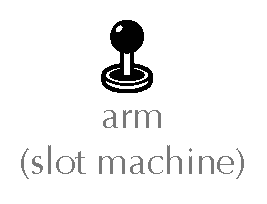
\includegraphics[scale=0.6]{fig/single-1}
    \end{subfigure}
    }
    \only<2>
    {
    \begin{subfigure}[c]{0.9\textwidth}
      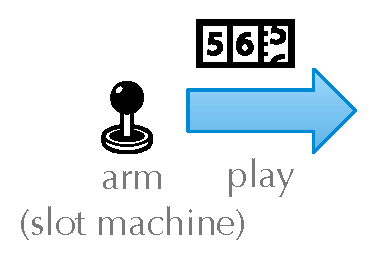
\includegraphics[scale=0.6]{fig/single-2}
    \end{subfigure}
    }
    \only<3>
    {
    \begin{subfigure}[c]{0.9\textwidth}
      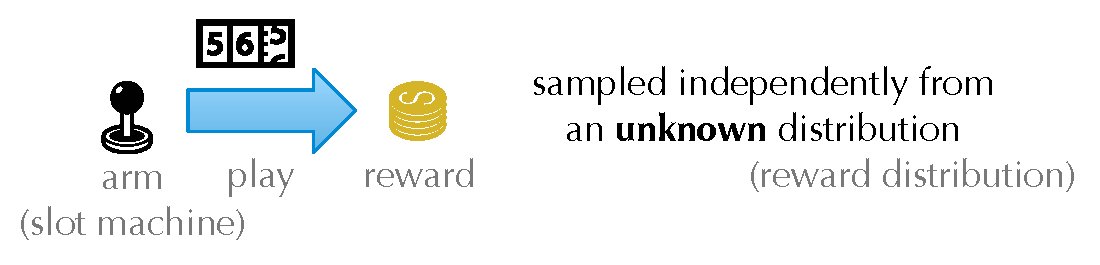
\includegraphics[scale=0.6]{fig/single-3}
    \end{subfigure}
    }
  \end{figure}
\end{frame}

\begin{frame}{Multi-armed bandit}
  \begin{columns}[T]
  \begin{column}[T]{0.5\textwidth}
  \begin{figure}
    \only<1>
    {
    \begin{subfigure}[c]{\textwidth}
      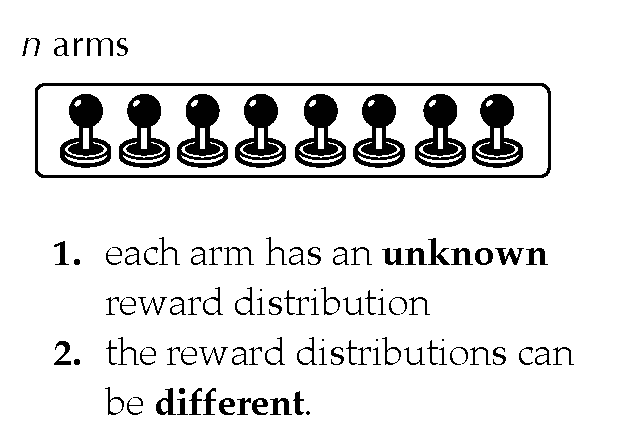
\includegraphics[scale=0.5]{fig/mab-1-1}
    \end{subfigure}
    }
    \only<2>
    {
    \begin{subfigure}[c]{\textwidth}
      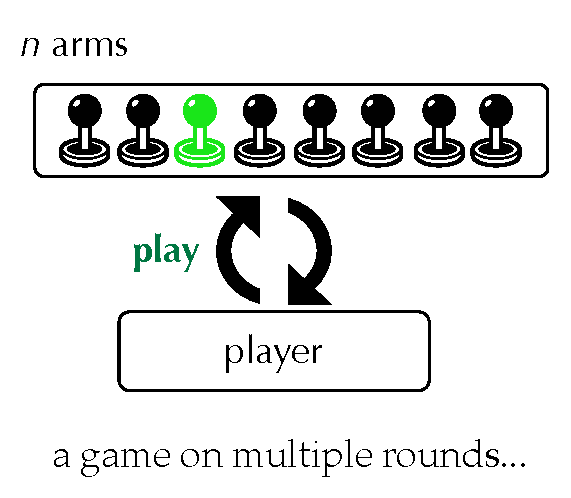
\includegraphics[scale=0.5]{fig/mab-s-1}
    \end{subfigure}
    }
    \only<3>
    {
    \begin{subfigure}[c]{\textwidth}
      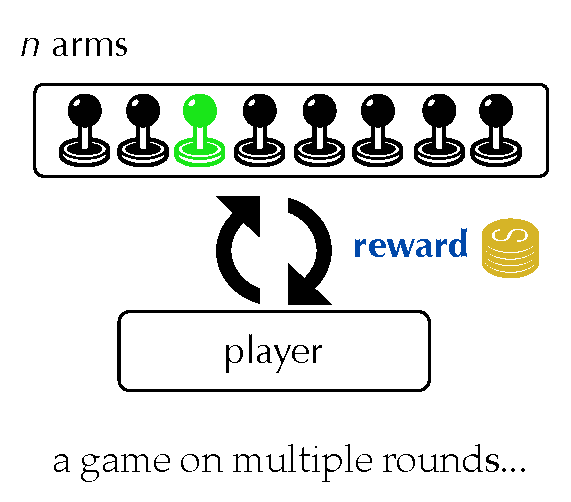
\includegraphics[scale=0.5]{fig/mab-s-1-2}
    \end{subfigure}
    }
    \only<4>
    {
    \begin{subfigure}[c]{\textwidth}
      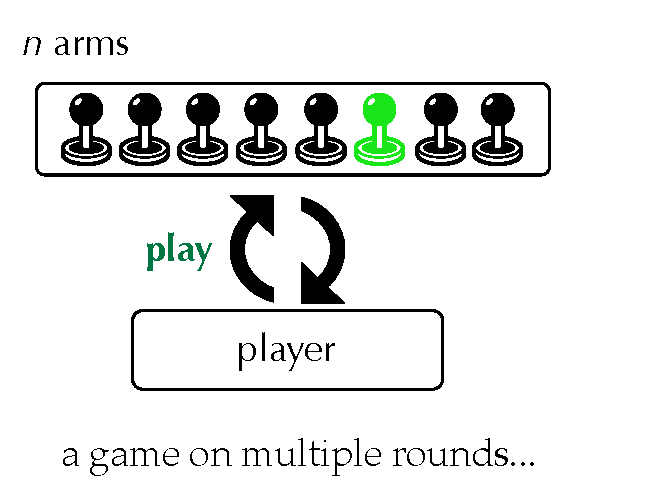
\includegraphics[scale=0.5]{fig/mab-s-2}
    \end{subfigure}
    }
    \only<5>
    {
    \begin{subfigure}[c]{\textwidth}
      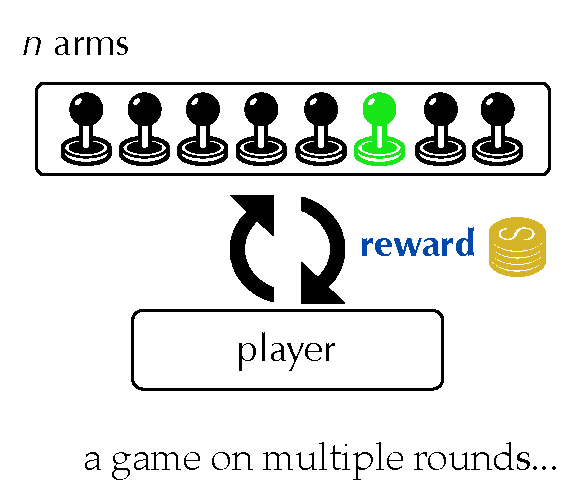
\includegraphics[scale=0.5]{fig/mab-s-2-2}
    \end{subfigure}
    }
    \uncover<6->
    {
    \begin{subfigure}[c]{\textwidth}
      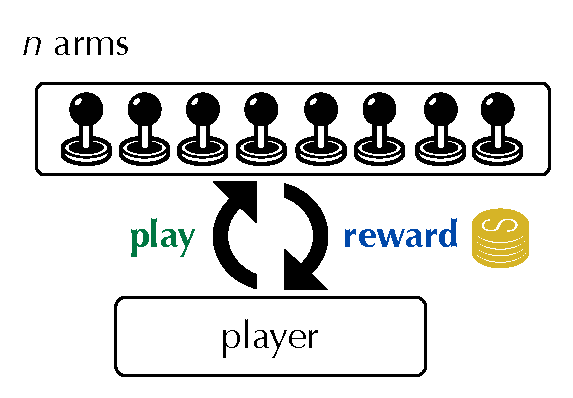
\includegraphics[scale=0.5]{fig/mab-1-0}
    \end{subfigure}
    }
    \uncover<7->
    {
    \begin{subfigure}[c]{\textwidth}
      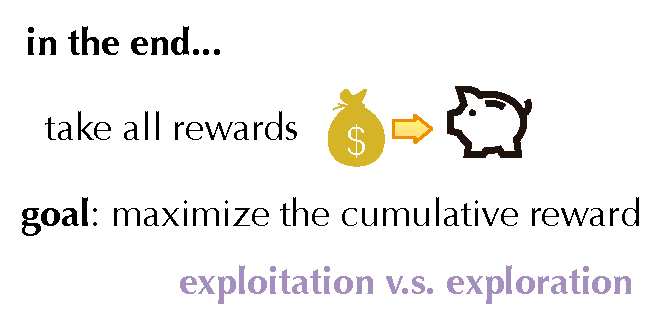
\includegraphics[scale=0.5]{fig/mab-1-3}
    \end{subfigure}    
    }
  \end{figure}
  \end{column}
  \begin{column}[T]{0.5\textwidth}
    \only<2-7>
    {
      \vspace{4em}
      \begin{exampleblock}{rules}
        for round $t = 1,\ldots, T$
        \begin{itemize}
          \item plays arm $i_t \in [n]$
          \item receives reward $X_{it} \sim \phi_{i}$
        \end{itemize}
      \end{exampleblock}
    }
  \begin{figure}
    \uncover<8->
    {
    \begin{subfigure}[c]{\textwidth}
      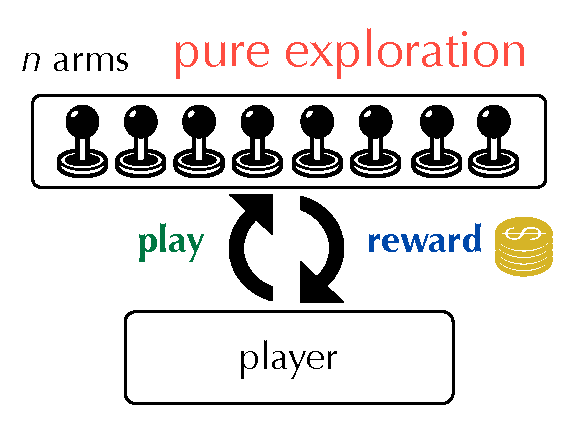
\includegraphics[scale=0.5]{fig/mab-2-1}
    \end{subfigure}
    }
  \end{figure}
  \end{column}
  \end{columns}
\end{frame}

\begin{frame}[noframenumbering]{Multi-armed bandit}
\begin{columns}
\begin{column}[t]{0.5\textwidth}
      \vspace{4em}
      \begin{exampleblock}{rules}
        for round $t = 1,\ldots, T$
        \begin{itemize}
          \item plays arm $i_t \in [n]$
          \item receives reward $X_{it} \sim \phi_{i}$
        \end{itemize}
      \end{exampleblock}

\end{column}
\begin{column}[t]{0.5\textwidth}
  \begin{figure}
    \begin{subfigure}[c]{\textwidth}
      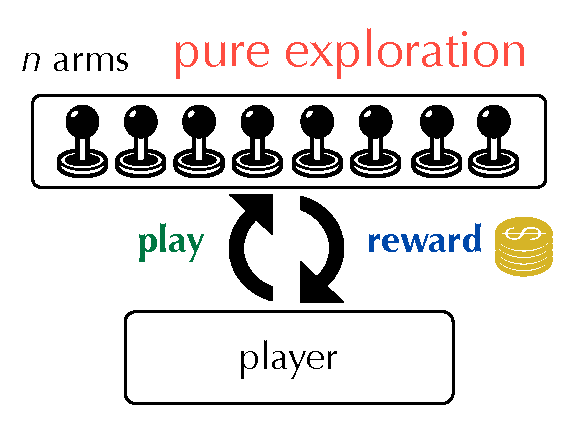
\includegraphics[scale=0.5]{fig/mab-2-1}
    \end{subfigure}
    \uncover<2->
    {
    \begin{subfigure}[c]{\textwidth}
      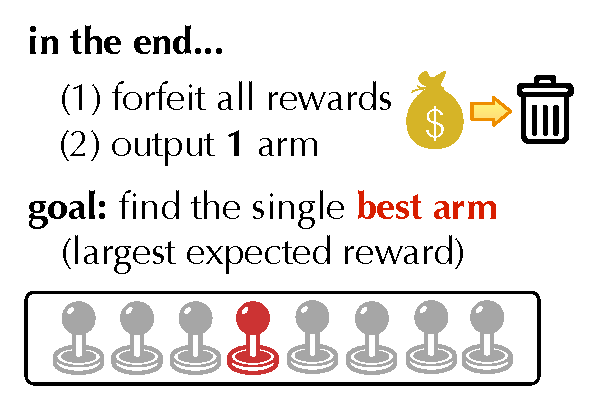
\includegraphics[scale=0.5]{fig/mab-2-2}
    \end{subfigure}    
    }
  \end{figure}
\end{column}
\end{columns}
\end{frame}

\begin{frame}{Pure Exploration of MAB}
  \textcolor{DarkBlue}{A/B testing, clinical trials, wireless network, crowdsourcing, ...}

  \begin{columns}
  \begin{column}[c]{0.3\textwidth}
  \begin{figure}
    \centering
    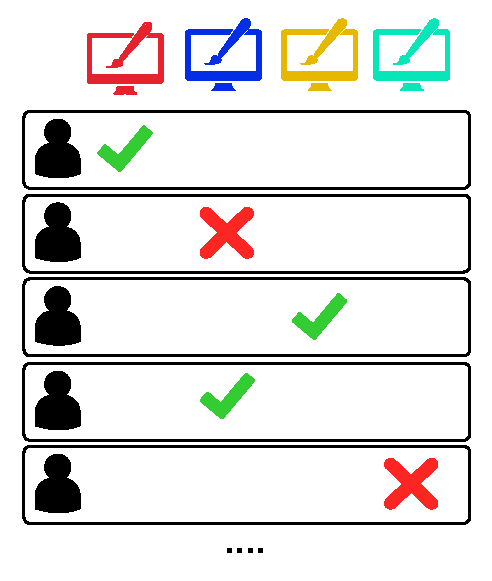
\includegraphics[scale=0.5]{fig/mt-2}
  \end{figure}  
  \end{column}
  \begin{column}[c]{0.7\textwidth}
    \vspace{2em}
    \begin{itemize}
      \item $n$ arms  = $n$ variants
      \item play arm $i$ = a page view on the $i$-th variant
      \item reward = a click on the ads
      \item finding the best arm = finding the variant with the highest average ads clicks
    \end{itemize}
  \end{column}
  \end{columns}
\end{frame}

\begin{frame}{Pure exploration: two settings}
\begin{columns}[t]
  \begin{column}[t]{0.5\textwidth}
    \begin{alertblock}{fixed budget}
      \begin{itemize}
        \item play for $T$ rounds.
        \item report the best arm after finished.
        \item \textbf{goal}: minimize the probability of error $\Pr[\text{out} \not= i_*]$
      \end{itemize}    
    \end{alertblock}
  \end{column}
  \begin{column}[t]{0.5\textwidth}
    \begin{alertblock}{fixed confidence}
      \begin{itemize}
        \item play for any number of rounds.
        \item report the best arm after finished
        \item guarantee that probability of error $\Pr[\text{out} \not= i_*] <\delta$.
        \item \textbf{goal}: minimize the number of rounds (\alert{sample complexity}).
      \end{itemize}
    \end{alertblock}
  \end{column}
\end{columns}

%\begin{columns}[t]
%  \begin{column}[t]{0.5\textwidth}
%    \begin{example}[medical trial]
%       find the best drug using 100 trials
%    \end{example}
%  \end{column}
%  \begin{column}[t]{0.5\textwidth}
%    \begin{example}[medical trial]
%      find the best drug with probability at least $0.9$ 
%      and use the smallest number of trials
%    \end{example}
%  \end{column}
%\end{columns}
\end{frame}

\begin{frame}{Combinatorial Pure Exploration of MAB}
  \begin{block}{Combinatorial Pure Exploration (CPE)}
    \vspace{-1em}
    \begin{itemize}
      \item play one arm at each round
      \item find the optimal \textbf{set} of arms $M_*$ satisfying certain constraint
      \vspace{-1em}
              $$M_* = \argmax_{\textcolor{DarkRed}{M\in \M}} \sum_{e \in M} w(e)$$
      \vspace{-1em}
      \begin{itemize}         
        \item $[n]$: set of arms
        \item $\M \subseteq 2^{[n]}$: \textcolor{DarkBlue}{decision class} with a combinatorial
        	constraint
        \item maximize the  \textcolor{DarkBlue}{sum of expected rewards} of arms in the set  
        %\item $\M \subseteq 2^{[n]}$ is the collection of valid sets.              
      \end{itemize}
    \end{itemize}
  \end{block} 
  \vspace{-1em}
  \begin{figure}[ht]
  \centering
  \begin{subfigure}[c]{0.40\textwidth}
    \caption{\textcolor{DarkBlue}{size-$k$-sets}}
    \centering
    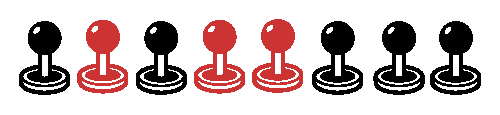
\includegraphics[scale=0.4]{fig/k-sets}
  \end{subfigure}
  ~
  \begin{subfigure}[c]{0.40\textwidth}
    \caption{\textcolor{DarkBlue}{spanning trees}}
    \centering
    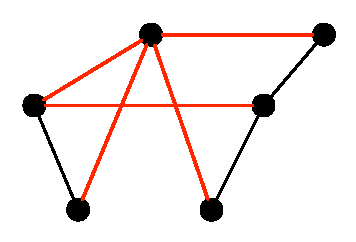
\includegraphics[height=3em]{fig/k-tree}
  \end{subfigure}
  ~
  \begin{subfigure}[c]{0.40\textwidth}
    \caption{\textcolor{DarkBlue}{paths}}
    \centering
    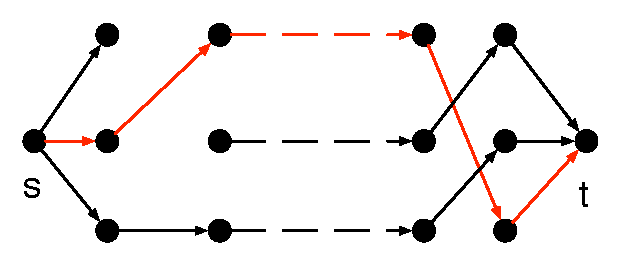
\includegraphics[height=3em]{fig/st-path}
  \end{subfigure}
  ~
  \begin{subfigure}[c]{0.40\textwidth}
    \caption{\textcolor{DarkBlue}{matchings}}
    \centering
    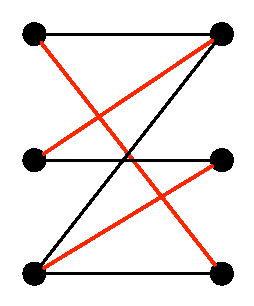
\includegraphics[height=3em]{fig/k-match}
  \end{subfigure}
  \end{figure}
\end{frame}


\begin{frame}{Motivating Examples}
  \begin{itemize}
    \item<1-> \textcolor{DarkRed}{matching}
      \begin{figure}
        %\centering
        \textcolor{black}{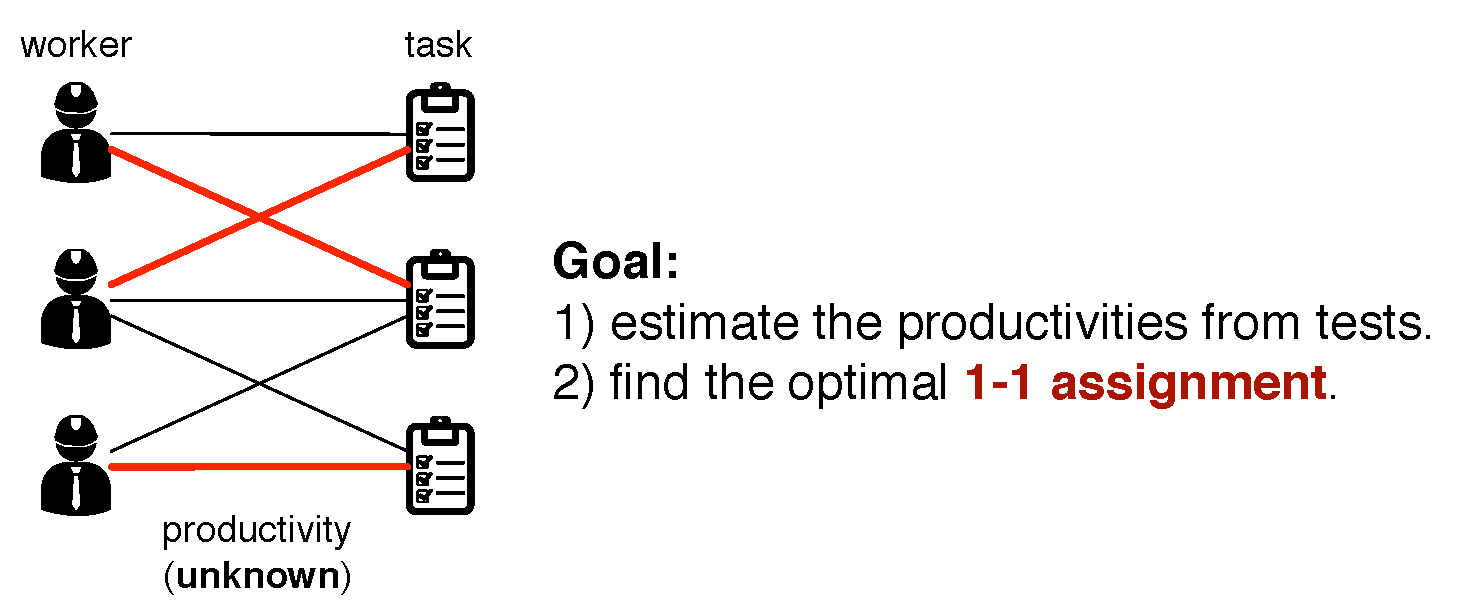
\includegraphics[height=8em]{fig/mot-match-2}}
      \end{figure}
    \item<2-> \textcolor{DarkRed}{spanning trees and paths}
      \begin{figure}
        %\centering
        \textcolor{black}{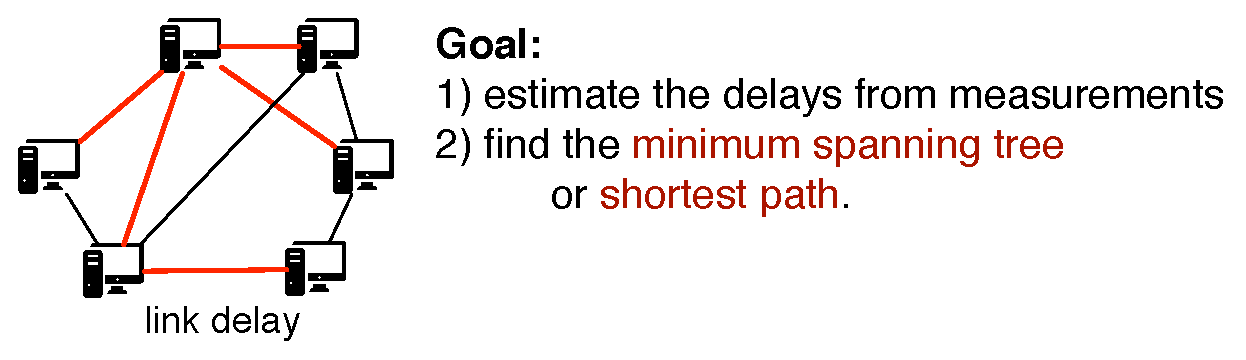
\includegraphics[height=6em]{fig/mot-tree}}
      \end{figure}    
    \item<3-> \textcolor{DarkRed}{size-$k$-sets}
      \begin{itemize}
        \item finding the top-$k$ arms.
      \end{itemize}      
  \end{itemize}
\end{frame}

\begin{frame}{Existing Work}
  \begin{itemize}
  %\textcolor{DarkRed}{known results} algorithms with matching lower bounds \textcolor{DarkBlue}{[JMNB14]}
    \item find top-$k$ arms \textcolor{DarkBlue}{[KS10,GGL12,KTPS12,BWV13,KK13,ZCL14]}
    \item find top arms in disjoint groups   of arms \textcolor{DarkBlue}{[GGLB11,GGL12,BWV13]}
    \item separate treatments, no unified framework
  \end{itemize}  
\end{frame}


\begin{frame}{Our Results}

  \begin{itemize}
    \item<2-> \textcolor{DarkRed}{general framework}
      \begin{itemize}
        \item for a wide range of combinatorial constraints $\M$.
      \end{itemize}
    \item<3-> \textcolor{DarkRed}{algorithms}
      \begin{itemize}
        \item two generic learning algorithms.
      \end{itemize}
    \item<4-> \textcolor{DarkRed}{upper bounds}
      \begin{itemize}
        \item sample complexity / probability of error.
        %\item \textbf{exchange class}: a new tool for analysis.
      \end{itemize}
    \item<5-> \textcolor{DarkRed}{lower bound}
      \begin{itemize}
        \item algorithms are \alert{optimal} (within log factors) for many types of $\M$ (in particular, bases of a matroid).
      \end{itemize}
    \item<6-> \textcolor{DarkRed}{compared with existing work}
      \begin{itemize}
        \item the first lower bound for the top-$k$ problem
        \item the first upper and lower bounds for other combinatorial constraints.
      \end{itemize}
  \end{itemize}  
\end{frame}

%\begin{frame}{Related Work}
%  \begin{itemize}
%    \item \textcolor{DarkRed}{Pure exploration of multi-armed bandits}
%      \begin{itemize}
%        \item finding the \textcolor{DarkBlue}{single best arm}: matching upper and lower bounds are known.
%        \item finding the \textcolor{DarkBlue}{top-$k$ arms}: only upper bounds are known.
%      \end{itemize}
%    \item<2-> \textcolor{DarkRed}{Combinatorial bandits}
%      \begin{itemize}
%        \item sets of arms are played at each round.
%        \item minimizing the \textcolor{DarkBlue}{cumulative regret}, instead of \textcolor{DarkBlue}{finding the best set}.
%          \begin{itemize}
%            \item \alert{the two problems are fundamentally different.}
%          \end{itemize}
%      \end{itemize}
%    \item<3-> \textcolor{DarkRed}{\textbf{Our results}}
%          \begin{itemize}
%            \item the first lower bound of top-$k$ problem.            
%            %\item Our upper bounds for top-$k$ problem match existing ones.
%            \item the first upper and lower bounds for other combinatorial constraints.
%          \end{itemize}      
%  \end{itemize}
%\end{frame}

\junk{
\begin{frame}{Two Settings}
  \begin{itemize}
    \item \textcolor{DarkRed}{Fixed budget}
      \begin{itemize}
        \item play for $T$ rounds.
        \item report the best set after finished.
        \item \textbf{goal}: minimize the probability of error
      \end{itemize}
    \item<2-> \textcolor{DarkRed}{Fixed confidence}
      \begin{itemize}
        \item play for any number of rounds.
        \item report the best set after finished
        \item guarantee that probability of error $<\delta$.
        \item \textbf{goal}: minimize the number of rounds (\alert{sample complexity}).
      \end{itemize}
  \end{itemize}
\end{frame}
}

\begin{frame}{CLUCB: Fixed confidence algorithm}
  \textcolor{DarkRed}{input}
  \begin{itemize}
    \item \textcolor{DarkBlue}{confidence}: $\delta \in (0,1)$
    \item access to a \textcolor{DarkBlue}{maximization oracle}: $\Oracle(\cdot): \mathbb R^{n} \rightarrow \M$
    \begin{itemize}
%      \item $\Oracle: \mathbb R^n\rightarrow \M$
      \item $\Oracle(v) = \argmax_{M\in \M} \sum_{i\in M} v(i)$ for \textcolor{DarkBlue}{weights} $v \in \RR^{n}$
    \end{itemize}
  \end{itemize}
  \textcolor{DarkRed}{output}
  \begin{itemize}
    \item a \textcolor{DarkBlue}{set} of arms: $M \in \M$.
  \end{itemize}
  %\textcolor{DarkRed}{algorithmic problems}
  %\begin{itemize}
  %  \item play which arm at each round?
  %  \item when to stop?
  %\end{itemize}
\end{frame}



\begin{frame}[noframenumbering]{CLUCB: Fixed confidence algorithm}
  \begin{figure}[ht]
  \centering
  \begin{subfigure}[c]{\textwidth}
    \hspace{3.5em}
    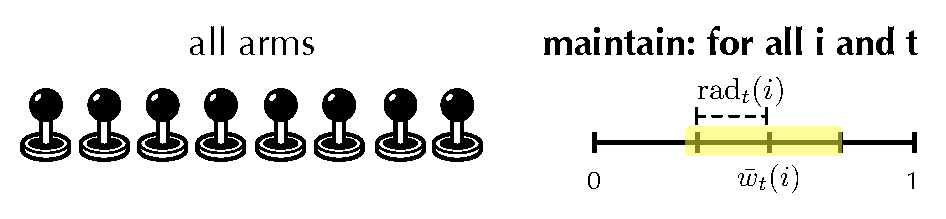
\includegraphics[scale=0.5]{fig/clucb-1}
  \end{subfigure}
  \end{figure}
  \begin{block}{notations}
  \begin{itemize}
    \item for each arm $i\in[n]$ in each round $t$
    \begin{itemize}
    \item empirical mean: $\bar w_t(i)$
    \item confidence radius: $\rad_t(i)$ \textcolor{Charcoal}{(proportional to $1/\sqrt{n_t(i)}$)}
    \end{itemize}
  \end{itemize}
  \end{block}
  \vspace{3.5em}
\end{frame}




\begin{frame}[noframenumbering]{CLUCB: Fixed confidence algorithm}
  \begin{figure}[ht]
  \centering
  \begin{subfigure}[c]{\textwidth}
    \hspace{3.5em}
    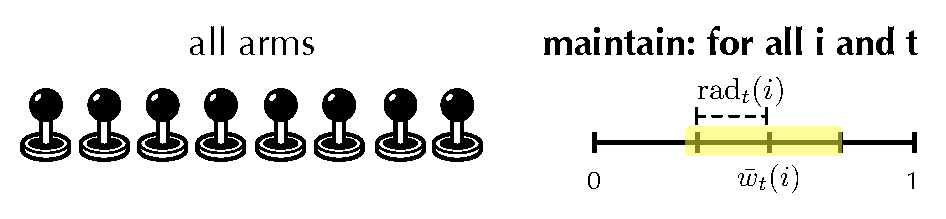
\includegraphics[scale=0.5]{fig/clucb-1}
  \end{subfigure}
  \begin{subfigure}[c]{\textwidth}
  \vspace{-1em}
    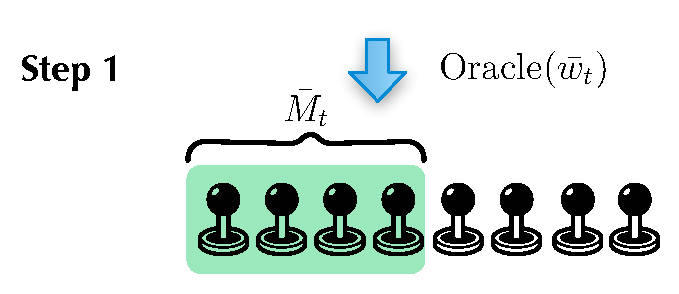
\includegraphics[scale=0.5]{fig/clucb-2}
  \end{subfigure}  
  \pause
  \begin{subfigure}[c]{\textwidth}
    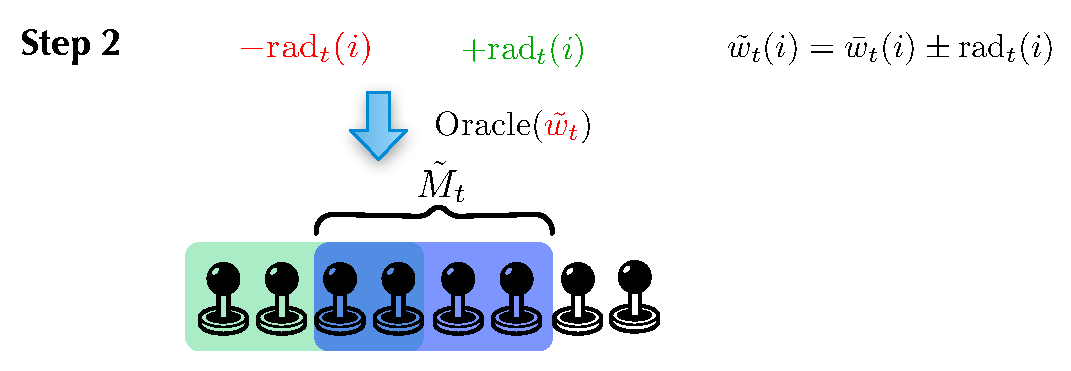
\includegraphics[scale=0.5]{fig/clucb-3}
  \end{subfigure}
  \end{figure}
\end{frame}


\begin{frame}[noframenumbering]{CLUCB: Fixed confidence algorithm}
  \begin{figure}[ht]
  \centering
  \begin{subfigure}[c]{\textwidth}
    \hspace{3.5em}
    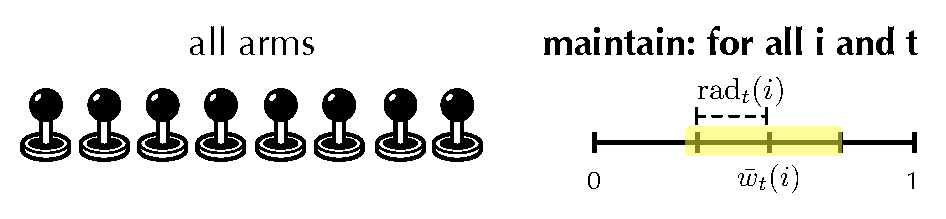
\includegraphics[scale=0.5]{fig/clucb-1}
  \end{subfigure}
  \begin{subfigure}[c]{\textwidth}
  \vspace{-1em}
    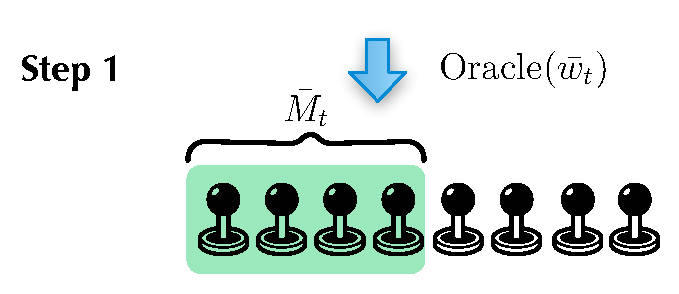
\includegraphics[scale=0.5]{fig/clucb-2}
  \end{subfigure}  
  \begin{subfigure}[c]{\textwidth}
    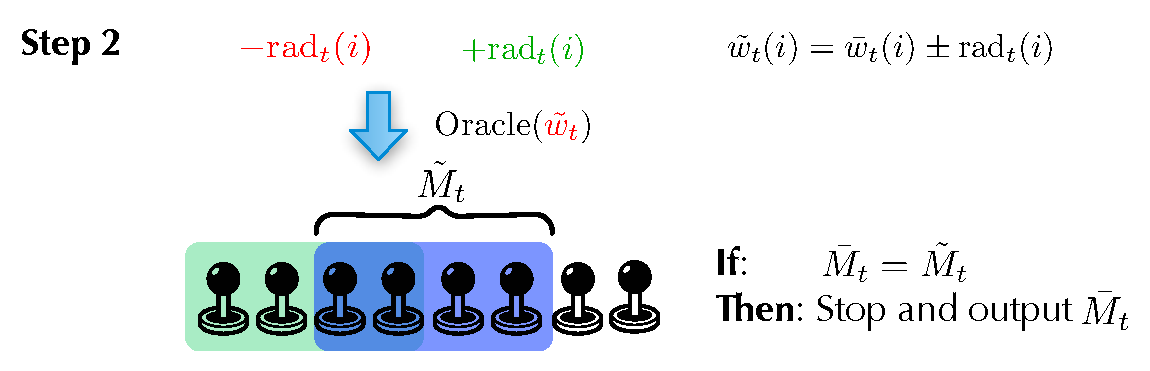
\includegraphics[scale=0.5]{fig/clucb-3-2}
  \end{subfigure}
  \end{figure}
\end{frame}


\begin{frame}[noframenumbering]{CLUCB: Fixed confidence algorithm}
  \begin{figure}[ht]
  \centering
  \begin{subfigure}[c]{\textwidth}
    \hspace{3.5em}
    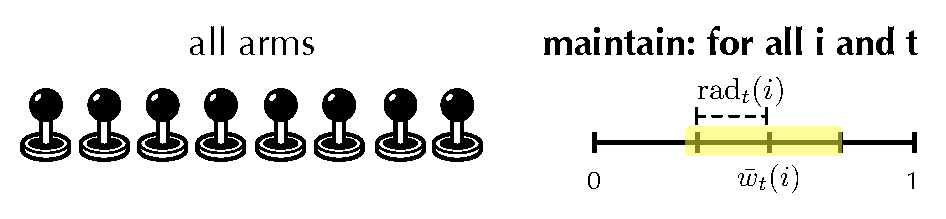
\includegraphics[scale=0.5]{fig/clucb-1}
  \end{subfigure}
  \begin{subfigure}[c]{\textwidth}
  \vspace{-1em}
    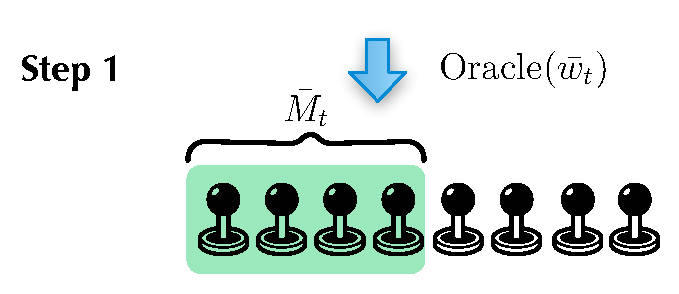
\includegraphics[scale=0.5]{fig/clucb-2}
  \end{subfigure}  
  \begin{subfigure}[c]{\textwidth}
    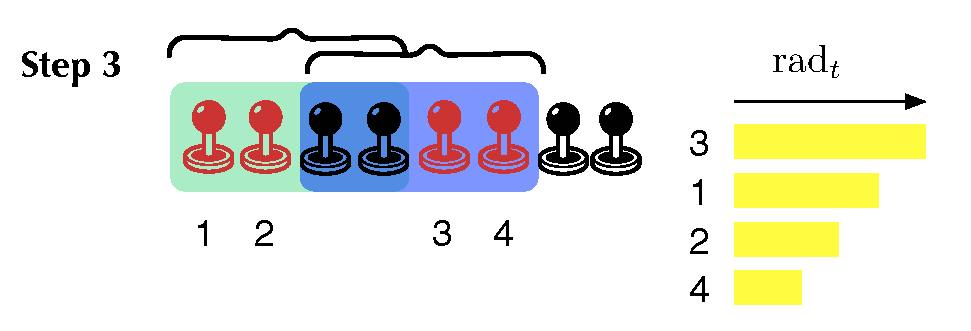
\includegraphics[scale=0.5]{fig/clucb-4}
  \end{subfigure}
  \end{figure}
\end{frame}

\begin{frame}[noframenumbering]{CLUCB: Fixed confidence algorithm}
  \begin{figure}[ht]
  \centering
  \begin{subfigure}[c]{\textwidth}
    \hspace{3.5em}
    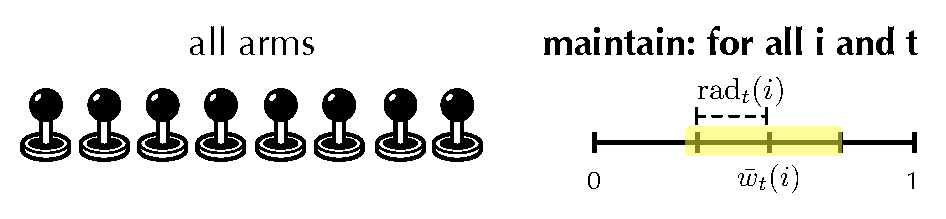
\includegraphics[scale=0.5]{fig/clucb-1}
  \end{subfigure}
  \begin{subfigure}[c]{\textwidth}
  \vspace{-1em}
    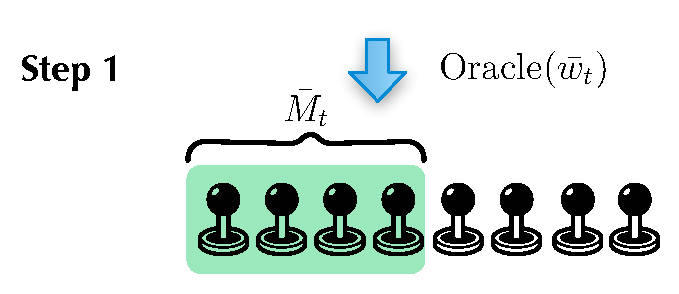
\includegraphics[scale=0.5]{fig/clucb-2}
  \end{subfigure}  
  \begin{subfigure}[c]{\textwidth}
    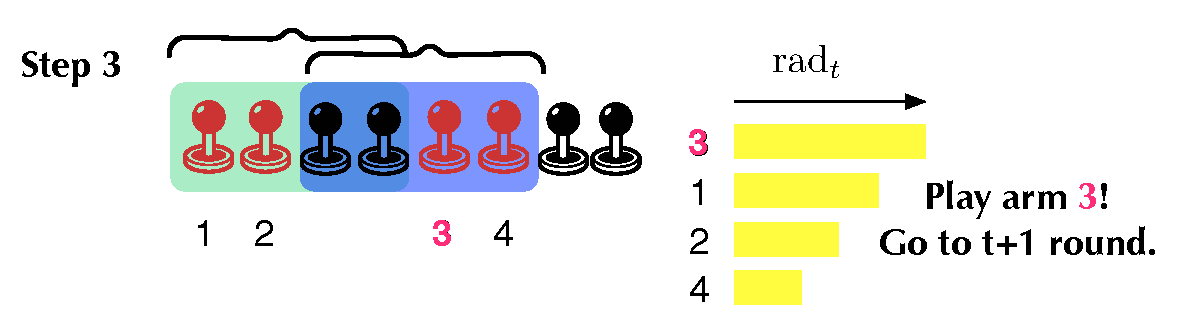
\includegraphics[scale=0.5]{fig/clucb-4-2}
  \end{subfigure}
  \end{figure}
\end{frame}

\begin{frame}{CLUCB: Sample Complexity}
\uncover<2->
{
\begin{theorem}[Upper bound]
  With probability at least $1-\delta$, CLUCB algorithm:
    \begin{enumerate} 
      \item correctly outputs the optimal set $M_*$
      \item uses at most $O(\textcolor{DarkRed}{\rank(\M)^2} \textcolor{DarkBlue}{\mathbf H} \log(n\mathbf H/\delta))$ rounds.
    \end{enumerate}
\end{theorem}
}

Our sample complexity bound depends on two quantities.
\begin{itemize}
  \item $\textcolor{DarkBlue}{\mathbf H}$:  depends on expected rewards
  \item $\textcolor{DarkRed}{\rank(\M)}$: depends on the structure of $\M$
\end{itemize}
\vspace{4em}
\end{frame}

\junk{
\begin{frame}{Results at a glance}
\begin{theorem}[Upper bound]
  With probability at least $1-\delta$, CLUCB algorithm:
    \begin{enumerate} 
      \item outputs the optimal set $M_* \triangleq \argmax_{M\in \M} w(M)$.
      \item uses at most $O(\textcolor{DarkRed}{\rank(\M)^2} \textcolor{DarkBlue}{\mathbf H} \log(n\mathbf H/\delta))$ rounds.
    \end{enumerate}
\end{theorem}
\begin{theorem}[Lower bound]
  Given any CPE instance, any $\delta$-correct algorithm must use at least $\Omega(\textcolor{DarkBlue}{\mathbf H} \log (1/\delta))$ rounds.
  \textcolor{Charcoal}{(An algorithm $\mathbb A$ is $\delta$-correct algorithm, if $\mathbb A$'s probability of error is at most $\delta$ for any instances)}
\end{theorem}
\pause
\begin{example}[Widths]
    \begin{itemize}
    \item \textbf{$k$-sets, spanning trees, bases of a matroid}: $\rank(\M) = 2$.
    \item \textbf{matchings, paths (in DAG)}:  $\rank(\M) = O(|V|)$.
    \item \textbf{in general}: $\rank(\M) \le n$
    \end{itemize}
\end{example}
\end{frame}
}

\begin{frame}{Results at a glance}
\begin{theorem}[Upper bound]
  With probability at least $1-\delta$, CLUCB algorithm:
    \begin{enumerate} 
      \item outputs the optimal set $M_* \triangleq \argmax_{M\in \M} w(M)$.
      \item uses at most $O(\textcolor{DarkRed}{\rank(\M)^2} \textcolor{DarkBlue}{\mathbf H} \log(n\mathbf H/\delta))$ rounds.
    \end{enumerate}
\end{theorem}
\begin{theorem}[Lower bound]
  Given any expected rewards, any $\delta$-correct algorithm must use at least $\Omega(\textcolor{DarkBlue}{\mathbf H} \log (1/\delta))$ rounds.
  \textcolor{Charcoal}{(An algorithm $\mathbb A$ is $\delta$-correct algorithm, if $\mathbb A$'s probability of error is at most $\delta$ for any instances)}
\end{theorem}
\begin{example}[Sample Complexities]
    \begin{itemize}
    \item \textbf{$k$-sets, spanning trees, bases of a matroid}: $\tilde O(\textcolor{DarkBlue}{\mathbf H})$ \alert{optimal!} 
    \item \textbf{matchings, paths (in DAG)}:  $\tilde O(\textcolor{DarkRed}{|V|^2}\textcolor{DarkBlue}{\mathbf H})$.
    \item \textbf{in general}: $\tilde O(\textcolor{DarkRed}{n^2}\textcolor{DarkBlue}{\mathbf H})$
    \end{itemize}
\end{example}
\end{frame}


\begin{frame}{$\mathbf H$ and gaps}
  \begin{itemize}
    \item $\Delta_e$: \alert{gap} of arm $e\in [n]$
        \begin{equation*}
          \Delta_e = \begin{cases}
             w(M_*)-\max_{M\in \M: e\in M} w(M) & \text{if } e\not \in M_*, \\
             w(M_*)-\max_{M\in \M: e\not \in M} w(M) & \text{if } e\in M_*
          \end{cases}
        \end{equation*}
        \begin{itemize}
           \item stability of the optimality of $M_*$ wrt. arm $e$.
        \end{itemize}
    \item
      $\textcolor{DarkBlue}{\mathbf H} =\sum_{e\in [n]} \Delta_e^{-2}$
      \begin{itemize}
        \item for the \textcolor{DarkRed}{top-$K$} problem: recover the previous definition of $\textcolor{DarkBlue}{\mathbf H}$.
      \end{itemize}
  \end{itemize}
\end{frame}


\begin{frame}{Width and exchange class}
  \begin{exampleblock}{Intuitions}
    \begin{itemize}
      \item we need a unifying method of analyzing different $\M$
      \begin{itemize}
        \item an \textcolor{DarkBlue}{exchange class} is a ``proxy'' for the structure of $\M$.
      \end{itemize}
      \item an exchange class $\B$ is a collection of ``patches'' ($(b_+,b_-), b_+,b_-\subseteq [n]$) that are used to interpolate between valid sets
      ($M\setminus b_- \cup b_+ = M', M,M' \in \M$).
%      \item width is the largest size of patches.
    \end{itemize}
  \end{exampleblock}
\begin{figure}[ht]
\centering
\begin{subfigure}[t]{0.22\textwidth}
  \caption{\textcolor{DarkBlue}{size-$k$-sets}}
  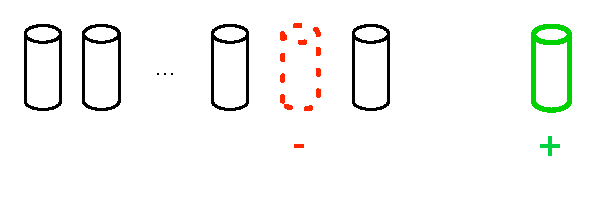
\includegraphics[width=\textwidth]{fig/exchange-multi}
  \label{fig:exchange:topk} 
\end{subfigure}
~
\begin{subfigure}[t]{0.22\textwidth}
  \caption{\textcolor{DarkBlue}{spanning tree}}
  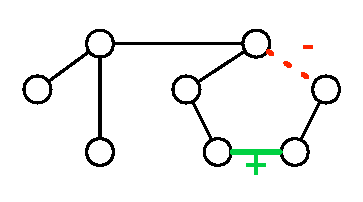
\includegraphics[width=\textwidth]{fig/exchange-matroid}
  \label{fig:exchange:matroid}
\end{subfigure}
~
\begin{subfigure}[t]{0.22\textwidth}
  \caption{\textcolor{DarkBlue}{matching}}
  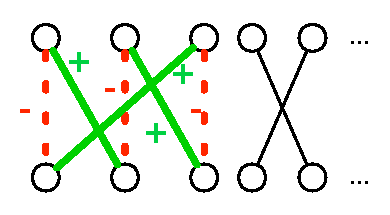
\includegraphics[width=\textwidth]{fig/exchange-match}
\end{subfigure}
~
\begin{subfigure}[t]{0.22\textwidth}
  \caption{\textcolor{DarkBlue}{path}}
  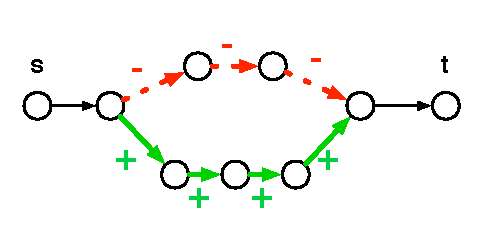
\includegraphics[width=\textwidth]{fig/exchange-path}
\end{subfigure}
\label{fig:exchange}
\end{figure}

\end{frame}



\begin{frame}{Width and exchange class}
\begin{columns}[T]
\begin{column}[t]{0.7\textwidth}
  \begin{exampleblock}{definition}
    %Let $\mathcal B$ be an exchange class. 
  \textcolor{DarkRed}{$\rank(\B)$: } the size of the largest ``patch''
  \begin{equation*}
    \label{eq:width}
    \rank(\B) = \max_{(b_+,b_-) \in \B} |b_+|+|b_-|.
  \end{equation*}
  \end{exampleblock}
\end{column}
\begin{column}[t]{0.3\textwidth}
\begin{figure}[t]
  %\caption{\textcolor{DarkBlue}{matching}}
  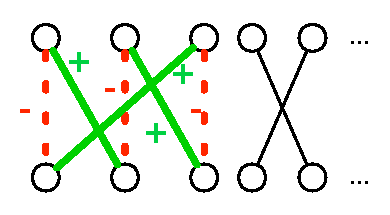
\includegraphics[width=\textwidth]{fig/exchange-match}
\end{figure}
\end{column}
\end{columns}
 % Let $\Exchange(\M)$ denote the family of all possible exchange classes for $\M$.
 % We define the width of $\M$ to be the width of the thinnest exchange class
\hspace{-5mm}
  \textcolor{DarkRed}{$\rank(\M)$: }  the width of the ``thinnest'' exchange class
\hspace{-15mm}
  \begin{equation*}
  \label{eq:width-class}
  \rank(\M) = \min_{\B \in \Exchange(\M)} \rank(\B),
  \end{equation*}
  %\begin{itemize}
  %\item $\Exchange(\M)$: possible exchange classes for $\M$.
  %\end{itemize}
\textcolor{DarkBlue}{The main technical contribution: Define exchange class and its algebra and
	conduct generic analysis using exchange classes.}
\begin{example}[Widths]
    \begin{itemize}
    \item \textbf{$k$-sets, spanning trees, bases of a matroid}: $\rank(\M) = 2$.
    \item \textbf{matchings, paths (in DAG)}:  $\rank(\M) = O(|V|)$.
    \item \textbf{in general}: $\rank(\M) \le n$
    \end{itemize}
\end{example}
  
\end{frame}

\junk
{
\begin{frame}{Sample complexity of examples}
Recall that
\begin{theorem}
  With probability at least $1-\delta$, CLUCB algorithm:
    \begin{enumerate} 
      \item outputs the  optimal set $M_*$.
      \item uses at most $\tilde O({\rank(\M)^2} {\mathbf H})$ rounds.
    \end{enumerate}
\end{theorem}
\pause
Plug in the widths of examples
\begin{corollary}[Sample Complexity of Examples]
    \begin{itemize}
    \item \textcolor{DarkBlue}{$k$-sets, spanning trees, bases of a matroid}: $\tilde O(\mathbf H)$.
    \item \textcolor{DarkBlue}{matchings, paths (in DAG)}:  $\tilde O(|V|^2 \mathbf H)$.
    \end{itemize}
\end{corollary}
\end{frame}
}

\junk{
\begin{frame}{Lower bound}
An algorithm $\mathbb A$ is a \textcolor{DarkBlue}{$\delta$-correct algorithm}, if $\mathbb A$'s probability of error is at most $\delta$ for any expected rewards.
\pause
\begin{theorem}[Problem dependent lower bound]
  Given any expected rewards, any $\delta$-correct algorithm must use at least $\Omega(\mathbf H \log (1/\delta))$ rounds.
\end{theorem}
\pause
\textbf{Remarks:}
\begin{itemize}
\item \textcolor{DarkBlue}{$k$-sets, spanning trees, bases of a matroid}: CLUCB's sample complexity $\tilde O(\mathbf H)$ is \alert{optimal} (up to log factors).
\item \textcolor{DarkRed}{other $\M$ in general}: a gap of $\tilde O(\rank(\M)^2 ) = \tilde O(n^2)$.
\end{itemize}
\end{frame}
}

\begin{frame}{CSAR: Fixed budget algorithm}
  \textcolor{DarkRed}{input}
  \begin{itemize}
    \item \textcolor{DarkBlue}{budget}: $T$ (play for at most $T$ rounds)
    \item access to a \textcolor{DarkBlue}{maximization oracle}
  \end{itemize}
  \textcolor{DarkRed}{output}
  \begin{itemize}
    \item a \textcolor{DarkBlue}{set} of arms: $M \in \M$.
  \end{itemize}
  \textcolor{DarkRed}{overview:}
  \begin{itemize}
    \item break the $T$ rounds into $n$ phases.
  \end{itemize}
\end{frame}


\begin{frame}[noframenumbering]{CSAR: Fixed budget algorithm}
  \begin{columns}[T]
    \begin{column}[T]{0.5\textwidth}
      \begin{figure}[ht]
        \begin{subfigure}[c]{\textwidth}
          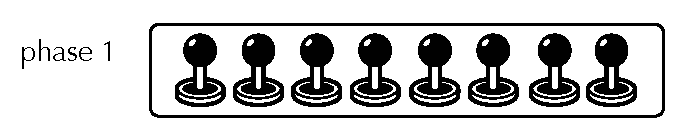
\includegraphics[scale=0.5]{fig/csar-0-1}
        \end{subfigure}
        \uncover<1->
        {
        \begin{subfigure}[c]{\textwidth}
          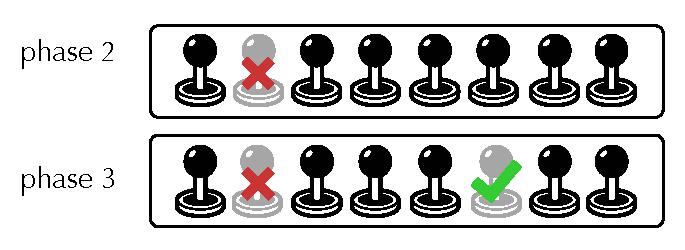
\includegraphics[scale=0.5]{fig/csar-0-2}
        \end{subfigure}  
        }
        \uncover<2->
        {
        \begin{subfigure}[c]{\textwidth}
          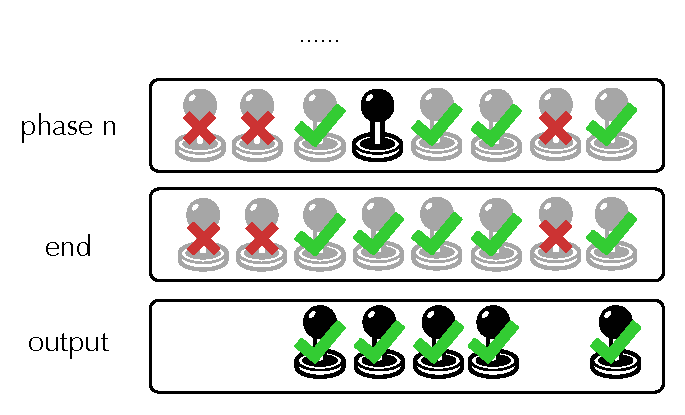
\includegraphics[scale=0.5]{fig/csar-0-3}
        \end{subfigure}
        }
      \end{figure}
    \end{column}
    \begin{column}[T]{0.5\textwidth}
      \uncover<1->
      {
      in each phase ($n$ phases in total):
      \begin{itemize}
        \item 1 arm is \textcolor{DarkGreen}{accepted} or \textcolor{DarkRed}{rejected}.
        \item \textcolor{DarkBlue}{active arms} are sampled for a same number of times.
      \end{itemize}
      \begin{figure}
        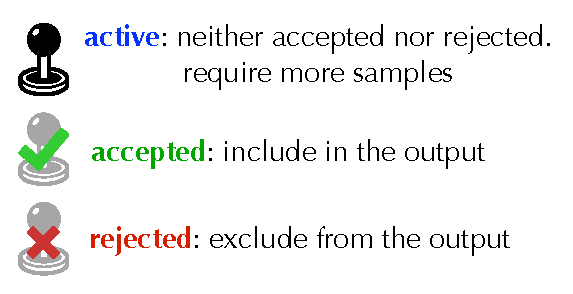
\includegraphics[scale=0.5]{fig/csar-0-4}
      \end{figure}
      }
      \only<3->
      { 
        \alert{problem:} which arm to accept or reject?
      }
    \end{column}
  \end{columns}
\end{frame}

\begin{frame}[noframenumbering]{CSAR: Fixed budget algorithm}
  \alert{problem:} which arm to accept or reject?

  \begin{itemize}
    \item accept/reject the arm with the largest \textbf{empirical gap}.
      $$
         \bar \Delta_e = \begin{cases}
            \bar w_t(\bar M_t)-{\max \atop M\in \M_t: e\in M} \bar w_t(M) & \text{if } e\not \in \bar M_t, \\
            \bar w_t(\bar M_t)-{\max \atop M\in \M_t: e\not \in M} \bar w_t(M) & \text{if } e\in \bar M_t
         \end{cases}
      $$
    \begin{itemize}
        \item $\M_t = \{M: M\in \M, \textcolor{DarkGreen}{A_t} \subseteq M, \textcolor{DarkRed}{B_t} \cap M = \emptyset\}$.
        \item $ \textcolor{DarkGreen}{A_t} $: accepted arms, $ \textcolor{DarkRed}{B_t}$: rejected arms (up to phase $t$).
        \item-> $\bar \Delta_e$ can be computed using a maximization oracle.
%        \item<2-> $\bar \Delta_e$ can be computed using a maximization oracle.        
    \end{itemize}
    \item-> recall the (unknown) \textbf{gap} of arm $e$:
      $$        
          \Delta_e = \begin{cases}
             w(M_*)-\max_{M\in \M: e\in M} w(M) & \text{if } e\not \in M_*, \\
             w(M_*)-\max_{M\in \M: e\not \in M} w(M) & \text{if } e\in M_*
          \end{cases}
      $$
  \end{itemize}
\end{frame}

\begin{frame}{CSAR: Probability of error}
\begin{theorem}[Probability of error of CSAR]
Given any budget $T>n$, CSAR correctly outputs the  optimal set $M_*$ with probability at least 
$$1 - 2^{\tilde O\left(-\frac{T}{\rank(\M)^2 \mathbf H} \right)}$$
and uses at most $T$ rounds.
\end{theorem}
\pause
\textcolor{DarkRed}{Remark:}
To guarantee  a constant  probability of error of $\delta$, both CSAR and CLUCB need $T=\tilde O(\rank(\M)^2 \mathbf H)$ rounds.
\end{frame}

\begin{frame}{Summary}
\begin{itemize}
  \item \textcolor{DarkBlue}{Combinatorial pure exploration}: a general framework that covers many pure exploration problems in MAB.
    \begin{itemize}
      \item find top-$k$ arms, optimal spanning trees, matchings or paths.
    \end{itemize}
  \item Two general algorithms (CLUCB, CSAR) for the problem
    \begin{itemize}
      \item only need a maximization oracle for $\M$.
      \item comparable performance guarantees.
    \end{itemize}
  \item Our algorithm is optimal (up to log factors) for matroids.
    \begin{itemize}
      \item including $k$-sets and spanning trees.
      %\item a  gap for other types of $\M$.
    \end{itemize}
  \item Trilogy on stochastic and combinatorial online learning : together with our recent work on 
  \textcolor{DarkBlue}{combinatorial multi-armed bandit} [CWY,ICML'13] and
  \textcolor{DarkBlue}{combinatorial partial monitoring} [LAKLC, ICML'14], 
  all dealing with general combinatorial
  constraints
\end{itemize}
\end{frame}

\begin{frame}{Future work}
\begin{itemize}
  \item Tighten the bounds for matching, paths and other combinatorial constraints
  \item Support approximation oracles
  \item Support non-linear reward functions
\end{itemize}
\end{frame}

\begin{frame}[plain]
\begin{center}
{
\Large
Thank you!

~\\

~\\

See you at Poster Wed2 tonight!
}
\end{center}
\end{frame}

\section{Backup}

\begin{frame}{Exchange class: Formal definition}
  \begin{block}{Exchange set}
     An \textbf{exchange set} $b$ is an ordered pair of disjoint sets $b=(b_+,b_-)$ where $b_+\cap b_- = \emptyset$ and $b_+,b_-\subseteq [n]$.

     Let $M$ be any set. We also define two operators:
     \begin{itemize}
        \item $M\oplus b \triangleq M\del b_- \cup b_+$.
        \item $M \ominus b \triangleq M\del b_+\cup b_-$.
     \end{itemize}
  \end{block}
  \begin{block}{Exchange class}
    We call a collection of exchange sets $\B$ an \textbf{exchange class for $\M$} if $\B$ satisfies the following property.
    For any $M,M'\in \M$ such that $M\not = M'$  and for any $e\in (M\del M')$, there exists an exchange set $(b_+,b_-)\in \B$ which satisfies five constraints: \textbf{(a)} $e\in b_-$, \textbf{(b)} $b_+ \subseteq M'\del M$, \textbf{(c)} $b_- \subseteq M \del M'$, \textbf{(d)} $(M\oplus b) \in \M$ and \textbf{(e)} $(M'\ominus b) \in \M$.
  \end{block}
\end{frame}

\begin{frame}{Experiments of CPE}
\begin{figure}
  \begin{subfigure}[c]{0.45\textwidth}
  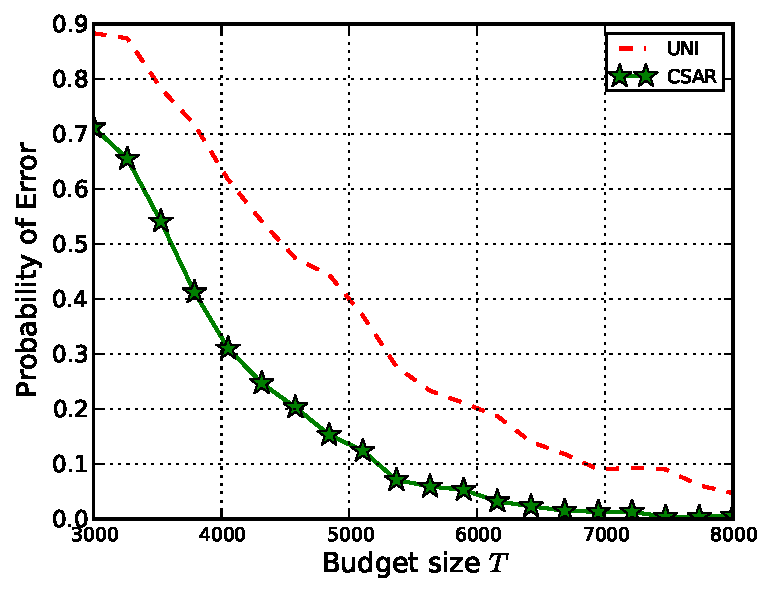
\includegraphics[width=\textwidth]{fig/mst-3257}
  \end{subfigure}
  \begin{subfigure}[c]{0.45\textwidth}
      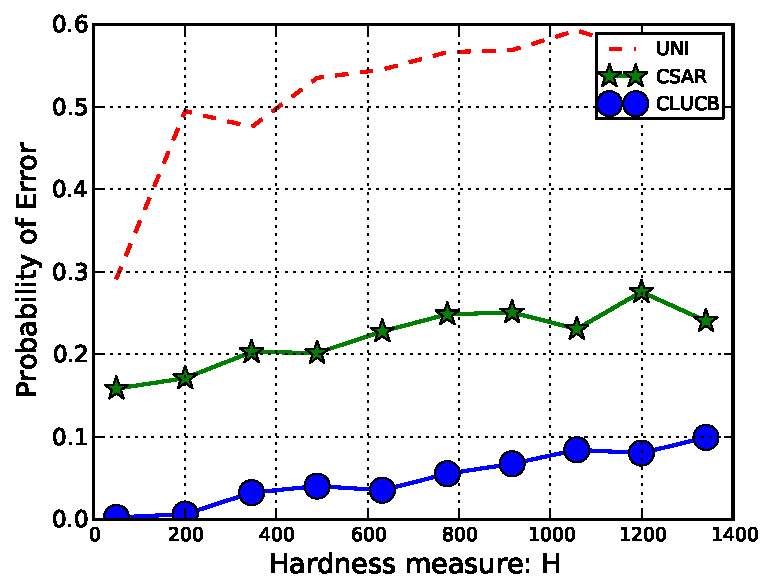
\includegraphics[width=\textwidth]{fig/mst-c-3257}
  \end{subfigure}
  \begin{subfigure}[c]{0.45\textwidth}
  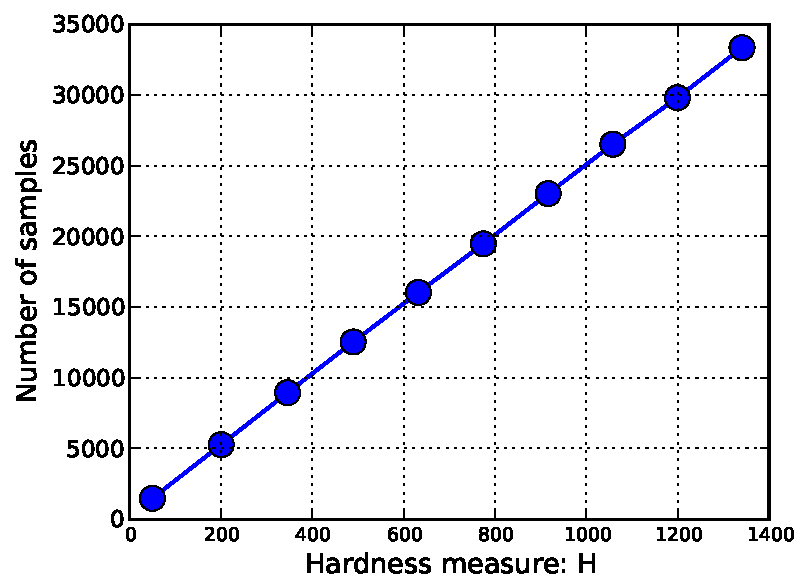
\includegraphics[width=\textwidth]{fig/mst-cs-3257}
  \end{subfigure}
\end{figure}
\end{frame}



\begin{frame}{Width and exchange class}
  \begin{exampleblock}{definition}

    Let $\mathcal B$ be an exchange class. 

  \begin{equation*}
    \label{eq:width}
    \rank(\B) = \max_{(b_+,b_-) \in \B} |b_+|+|b_-|.
  \end{equation*}
  
  Let $\Exchange(\M)$ denote the family of all possible exchange classes for $\M$.
  We define the width of $\M$ to be the width of the thinnest exchange class
  \begin{equation*}
  \label{eq:width-class}
  \rank(\M) = \min_{\B \in \Exchange(\M)} \rank(\B),
  \end{equation*}
  where $\Exchange(\M)$ is the family of all possible exchange classes for $\M$.
  \end{exampleblock}
  
\end{frame}

\end{document}
